\documentclass[conference]{IEEEtran}

% ── Packages ──────────────────────────────────────────────
\usepackage{cite}
\usepackage{amsmath,amssymb}
\usepackage{graphicx}
\usepackage{booktabs}
\usepackage{hyperref}
\usepackage{algorithm}
\usepackage{algpseudocode}
\usepackage{array}

% ── Title ─────────────────────────────────────────────────
\begin{document}

\title{PyVRP-Web: Bio-inspired Vehicle Routing Optimization\\
with Interactive Web Visualization}

\author{
  \IEEEauthorblockN{Student ID: 414085193}
  \IEEEauthorblockA{
    Department of Information Management\\
    National University of Science and Technology, Taiwan\\
    Email: 414085193@mail.ntust.edu.tw
  }
}

\maketitle

% ── Abstract ──────────────────────────────────────────────
\begin{abstract}
The Vehicle Routing Problem (VRP) is a combinatorial optimization problem
of high practical importance in logistics planning, yet it is NP-hard and
infeasible to solve optimally at scale. This paper presents our study of
PyVRP, a high-performance open-source VRP solver implementing Hybrid Genetic
Search (HGS)---a bio-inspired algorithm combining genetic evolution with
local search. We analyze the algorithmic components of HGS in depth,
including its SREX crossover operator, population diversity management via
Broken Pairs Distance, and adaptive penalty mechanism. Furthermore, we
implement PyVRP-Web, a full-stack web application that exposes the HGS
solver through an interactive browser interface, enabling zero-code problem
definition and real-time geographic route visualization. Benchmark evaluation
shows PyVRP achieves a mean gap of 0.22\% from best-known solutions on 100
CVRP instances, and 0.40\% on 60 VRPTW instances with 1,000 customers. A
real-world case study with 16 Taipei convenience stores validates practical
usability.
\end{abstract}

\begin{IEEEkeywords}
Vehicle Routing Problem, Hybrid Genetic Search, Genetic Algorithm,
Bio-inspired Computing, Web Application, Local Search
\end{IEEEkeywords}

% ── Section I: Introduction ───────────────────────────────
\section{Introduction}\label{sec:intro}

The \textbf{Vehicle Routing Problem (VRP)} is a classical combinatorial
optimization problem with direct applications in last-mile delivery, public
transit, and supply chain management. Given a depot, a fleet of vehicles
with limited capacity, and a set of customers with delivery demands, the VRP
seeks a minimum-cost set of routes such that every customer is served exactly
once and vehicle capacity constraints are satisfied~\cite{toth2014vehicle}.
The VRP with Time Windows (VRPTW) additionally requires each customer to be
served within a specified time interval.

VRP is NP-hard: for a problem with merely 20 customers, the number of
possible route permutations exceeds $2\times10^{18}$, making brute-force
enumeration computationally infeasible. This motivates the use of
\textbf{bio-inspired metaheuristics}---algorithms modeled on natural
processes such as evolutionary selection and genetic recombination---which
trade optimality guarantees for scalability.

This work centers on \textbf{PyVRP}~\cite{wouda2024pyvrp}, a
state-of-the-art solver implementing \textbf{Hybrid Genetic Search (HGS)}:
a framework synergizing Genetic Algorithm (GA) exploration with Local Search
exploitation. PyVRP won the 2021 DIMACS VRPTW Challenge and ranked first in
the EURO meets NeurIPS 2022 competition.

Our contributions are:
\begin{enumerate}
  \item \textbf{Algorithmic Analysis}: A systematic study of HGS components,
    including SREX crossover~\cite{nagata2010memetic}, broken pairs distance
    diversity, and adaptive penalty management.
  \item \textbf{System Implementation}: PyVRP-Web, a full-stack web
    application wrapping HGS in a zero-code interface with real-time map
    visualization. We identify three concrete barriers preventing practitioners
    from using research-grade VRP solvers: (i) the requirement to write Python
    code to assemble the solver model; (ii) the mismatch between PyVRP's
    integer planar coordinate system and real-world WGS84 GPS data; and
    (iii) the absence of visual route output. PyVRP-Web resolves all three.
\end{enumerate}

% ── Section II: Related Work ──────────────────────────────
\section{Related Work}

\subsection{VRP Solver Landscape}

Numerous tools address VRP. \textbf{LKH-3}~\cite{helsgaun2017extension}
transforms VRP into a TSP and applies the Lin-Kernighan heuristic, but is
restricted to academic, non-commercial use. \textbf{OR-Tools}~\cite{ortools}
from Google uses constraint programming and is easy to use but
performs far from the state of the art~\cite{wouda2024pyvrp}.
\textbf{VRPSolver}~\cite{pessoa2020generic} finds exact solutions but
does not scale beyond a few hundred customers. VROOM integrates with road
network APIs for real-world routing but lacks the solution quality of
HGS-based solvers.

PyVRP occupies a unique position: near-optimal performance comparable to
specialized C++ solvers, full Python customizability, and availability under
the MIT license.

\subsection{Hybrid Genetic Search}

HGS was introduced by Vidal et al.~\cite{vidal2013hybrid} for a broad class
of VRP variants, maintaining both feasible and infeasible solutions via
dynamic penalty coefficients. A key property is that this approach enables
exploration of a wider solution space while steering convergence toward
feasibility---an adaptive strategy inspired by environmental pressure in
natural evolution.

Vidal~\cite{vidal2022hybrid} extended HGS-CVRP with the SWAP* operator and
biased fitness criterion for population management. The SREX crossover
operator~\cite{nagata2010memetic} preserves complete sub-routes across
generations, avoiding the quality degradation of naive crossover operators
by inheriting intact high-quality route structures.

PyVRP~\cite{wouda2024pyvrp} builds on HGS-CVRP by adding VRPTW support,
adopting a Python+C++ hybrid architecture for extensibility, and
robustifying the implementation while maintaining competitive performance.

% ── Section III: Methods ──────────────────────────────────
\section{Methods}

\subsection{Problem Formulation}

The \textbf{CVRP} is defined on a complete directed graph $G=(V,A)$ where
$V=\{0,1,\ldots,n\}$ (0: depot, $1\ldots n$: customers). Customer $i$ has
demand $q_i\geq 0$; each vehicle has capacity $Q$. Objective:
\begin{equation}
  \min \sum_{(i,j)\in A} d_{ij}\,x_{ij}
\end{equation}
subject to every customer visited exactly once, routes starting/ending at
the depot, and total route demand $\leq Q$.

The \textbf{VRPTW} additionally requires service at customer $i$ to begin
within $[e_i, l_i]$, with service duration $s_i$ and travel time $t_{ij}$.
Vehicles may wait (if arriving early) but cannot violate the late deadline
$l_i$.

\subsection{Hybrid Genetic Search}

HGS~\cite{wouda2024pyvrp,vidal2013hybrid} is the core bio-inspired
algorithm. Its key insight is that neither GA nor Local Search alone performs
optimally---combining them yields superior results: GA provides
\textit{exploration} across the solution space while Local Search provides
\textit{exploitation} within promising regions.

The main loop is outlined in Algorithm~\ref{alg:hgs}.

\begin{algorithm}
\caption{HGS Main Loop}\label{alg:hgs}
\begin{algorithmic}[1]
\State Initialize population $\mathcal{P}$ with $n_{\min}=25$ random solutions
\State Set initial penalty weights ($\alpha=20$, $\beta=6$)
\Repeat
  \State $(p_1, p_2) \leftarrow$ \textsc{TournamentSelect}($\mathcal{P}$)
  \State $c \leftarrow$ \textsc{SREX}$(p_1, p_2)$
  \State $c \leftarrow$ \textsc{LocalSearch}$(c)$
  \If{$\text{rand}() < p_{\text{repair}}$ \textbf{and} infeasible($c$)}
    \State $c \leftarrow$ \textsc{LocalSearch}$(c,\ \alpha\times12,\ \beta\times12)$
  \EndIf
  \State $\mathcal{P} \leftarrow \mathcal{P} \cup \{c\}$
  \If{$|\mathcal{P}| > n_{\min} + n_{\text{gen}}$}
    \State \textsc{SurvivorSelection}($\mathcal{P}$)
  \EndIf
  \State \textsc{UpdatePenalties}($\mathcal{P}$) \Comment{every 50/100 iters}
\Until{stopping criterion met}
\State \Return best feasible solution
\end{algorithmic}
\end{algorithm}

\subsubsection{SREX Crossover}
The Selective Route Exchange operator~\cite{nagata2010memetic} constructs
an offspring by (1) inheriting a subset of complete routes from parent $B$,
then (2) greedily inserting unserved customers guided by parent $A$'s
structure. This preserves entire high-quality sub-routes across generations,
mimicking chromosomal recombination in biological evolution---where intact
functional gene segments are inherited rather than random base-pair mixtures.

\subsubsection{Local Search}
Local search~\cite{wouda2024pyvrp} accounts for \textbf{80--90\% of
runtime} and is implemented in C++. It operates at two levels:

\textit{Node operators} evaluate moves between customer pairs $(u,v)$ within
the \textbf{granular neighbourhood}~\cite{toth2003granular} of size $k$
(CVRP: $k=20$; VRPTW: $k=40$), reducing complexity from $O(n^2)$ to
$O(kn)$. PyVRP provides 11 operators: $(N,M)$-exchange for
$N\in\{1,2,3\}$, $M\leq N$ (implemented via C++ template specialization),
MoveTwoClientsReversed, and 2-OPT.

\textit{Route operators} evaluate cross-route moves: RELOCATE* (best
single-customer relocation) and SWAP* (best customer swap with optimal
insertion position, enhanced with time-window caching and early
termination~\cite{wouda2024pyvrp}).

\subsubsection{Population Management and Diversity}
The population maintains two sub-populations: \textit{feasible} and
\textit{infeasible} solutions. The biased fitness
criterion~\cite{vidal2022hybrid} balances quality and diversity---analogous
to natural selection favouring both fitness and genetic diversity within a
species:
\begin{equation}
  f_{\text{biased}}(s)=r_{\text{qual}}(s)\cdot(1-\rho)+r_{\text{div}}(s)\cdot\rho
\end{equation}
where $\rho = n_{\text{elite}}/n_{\min} = 4/25$ and diversity is measured
by \textbf{Broken Pairs Distance (BPD)}:
\begin{equation}
  \text{BPD}(A,B)=\frac{|P_A \triangle P_B|}{2n},\quad \text{BPD}\in[0,1]
\end{equation}
Survivor selection removes duplicates, then eliminates solutions with worst
biased fitness until the population returns to $n_{\min}=25$.

\subsubsection{Dynamic Penalty Management}
Constraints are treated as soft via penalized cost:
\begin{equation}
  c_{\text{pen}} = d_{\text{total}} + \alpha\,\Delta_{\text{cap}} + \beta\,\Delta_{\text{tw}}
\end{equation}
$\alpha$ and $\beta$ are dynamically adjusted every 50 iterations to
maintain a target feasibility ratio of 43\%. This adaptive mechanism acts
as an \textit{environmental pressure} in the evolutionary metaphor: when
too few solutions are feasible, constraints are tightened; when too many
are feasible, constraints are relaxed to encourage exploration. A repair
booster multiplies penalties by 12 when attempting to recover infeasible
offspring.

\begin{table}[h]
\caption{Key HGS Parameters}\label{tab:params}
\centering
\begin{tabular}{lll}
\toprule
\textbf{Parameter} & \textbf{Value} & \textbf{Description} \\
\midrule
$n_{\min}$ (min\_pop\_size) & 25 & Minimum population size \\
$n_{\text{gen}}$ (generation\_size) & 40 & New offspring per generation \\
$n_{\text{elite}}$ (nb\_elite) & 4 & Elite individuals \\
$k$ nb\_granular (CVRP) & 20 & Neighbour search radius \\
$k$ nb\_granular (VRPTW) & 40 & Neighbour search radius \\
target\_feasible & 43\% & Target feasibility ratio \\
Repair booster & $\times$12 & Penalty multiplier for repair \\
\bottomrule
\end{tabular}
\end{table}

\subsection{System Architecture: PyVRP-Web}

We designed and implemented PyVRP-Web, a four-layer full-stack
application (Figure~\ref{fig:arch}):
\begin{enumerate}
  \item \textit{Presentation}: Vanilla JS + Leaflet.js interactive map
  \item \textit{API}: FastAPI with Pydantic validation and
    \texttt{asyncio.Semaphore(1)} for concurrency control
  \item \textit{Service}: WGS84$\to$UTM coordinate conversion via pyproj
    (EPSG:32651), neighbourhood tuning ($k=\min(7,n{-}1)$), per-stop
    timeline reconstruction
  \item \textit{Engine}: PyVRP v0.5.0 HGS solver (unmodified black-box)
\end{enumerate}

\begin{figure}[t]
  \centering
  \includegraphics[width=\columnwidth]{figures/fig1_hgs_flowchart}
  \caption{Main loop of Hybrid Genetic Search (HGS). The algorithm
           combines genetic crossover (SREX), local search, and dynamic
           penalty management to explore and exploit the solution space.}
  \label{fig:hgs}
\end{figure}

\textbf{Design Principle---Zero-Intrusion Encapsulation}: PyVRP is treated
as an unmodified black-box library. All extensions are encapsulated in
surrounding service modules (\texttt{coord.py}, \texttt{solver.py},
\texttt{serializer.py}), ensuring that future PyVRP version upgrades require
no changes to the HGS core.

Three key engineering decisions resolved the three practitioner barriers
identified in Section~\ref{sec:intro}:

\textbf{(1) Coordinate Conversion}: PyVRP requires integer planar
coordinates. We project WGS84 latitude/longitude to UTM Zone 51N
(EPSG:32651) via pyproj, then scale by 10 to achieve 0.1-meter integer
precision with no metric distortion at Taiwan's latitude.

\textbf{(2) Neighbourhood Tuning}: PyVRP's default $k=20$ becomes
near-exhaustive for small problems (e.g., 16 customers), causing prohibitively
slow local search. We reduce it dynamically to $\min(7,n{-}1)$, enabling an
order-of-magnitude more iterations within the same wall-clock budget.

\textbf{(3) Per-Stop Timeline Reconstruction}: PyVRP's \texttt{Route}
object provides only the customer visit sequence. We reconstruct arrival and
departure times via forward simulation:
$t_{\text{arr}}^{i+1} = t_{\text{dep}}^i + t_{i,i+1}$, where
$t_{\text{dep}}^i = \max(t_{\text{arr}}^i,\, e_i) + s_i$.

% ── Section IV: Results ───────────────────────────────────
\section{Results}

\subsection{Benchmark Performance}

We evaluate PyVRP v0.5.0 on two standard benchmark sets following~\cite{wouda2024pyvrp}.

\begin{table}[h]
\caption{CVRP Benchmark Results (X instances~\cite{uchoa2017new}, 100 instances, 10 seeds)}
\label{tab:cvrp}
\centering
\begin{tabular}{lccc}
\toprule
\textbf{Solver} & \textbf{Mean Cost} & \textbf{Mean Gap} & \textbf{Gap of Mean} \\
\midrule
BKS             & 63,106.7 & 0.00\% & 0.00\% \\
HGS-CVRP~\cite{vidal2022hybrid} & 63,206.1 & 0.11\% & 0.16\% \\
HGS-2012~\cite{vidal2013hybrid} & 63,285.8 & 0.21\% & 0.28\% \\
\textbf{PyVRP~\cite{wouda2024pyvrp}} & \textbf{63,275.5} & \textbf{0.22\%} & \textbf{0.27\%} \\
\bottomrule
\end{tabular}
\end{table}

PyVRP achieves a mean gap of \textbf{0.22\%} from best-known solutions on
100 CVRP instances with 100--1001 customers ($T_{\max}=n\times2.4$\,s,
10 seeds). Multiple small-scale instances are solved to \textbf{proven
optimality} (0\% gap), e.g., X-n101-k25, X-n110-k13, X-n115-k10.

\begin{table}[h]
\caption{VRPTW Benchmark Results (H\&G 1000-customer instances~\cite{homberger1999two}, 60 instances)}
\label{tab:vrptw}
\centering
\begin{tabular}{lccc}
\toprule
\textbf{Solver} & \textbf{Mean Cost} & \textbf{Mean Gap} & \textbf{Gap of Mean} \\
\midrule
BKS              & 33,143.8 & 0.00\% & 0.00\% \\
HGS-DIMACS~\cite{kool2022hybrid} & 33,265.5 & 0.32\% & 0.37\% \\
\textbf{PyVRP~\cite{wouda2024pyvrp}} & \textbf{33,296.4} & \textbf{0.40\%} & \textbf{0.46\%} \\
\bottomrule
\end{tabular}
\end{table}

On 60 VRPTW instances with 1,000 customers (2-hour time limit, 10 seeds),
PyVRP achieves \textbf{0.40\%} mean gap---equivalent to a
\textbf{2nd-place rank} in the DIMACS VRPTW competition. In extended runs,
PyVRP improved \textbf{27 of 300} best-known solutions across the full H\&G
benchmark set. Performance varies by instance type: clustered instances with
wide time windows (C2) yield near-optimal results ($\approx$0.04\% gap),
while random instances with narrow time windows (R1, RC1) are more
challenging ($\approx$0.72\% gap).

\subsection{System Demonstration}

We validate PyVRP-Web on a real-world case study: \textbf{Taipei 7-ELEVEN
daytime distribution} (Figure~\ref{fig:webdemo}).

\textbf{Setup}: 1 depot (Unified Enterprise Taipei Distribution Center,
09:30--13:00), 16 stores across Taipei City (time windows 10:00--13:00),
2 large trucks (capacity 140) + 4 medium trucks (capacity 80), average
speed 28\,km/h.

\textbf{Results}: The HGS solver finds a feasible routing plan in
approximately \textbf{8 seconds} using \texttt{TimedNoImprovement(max\_iterations=500)}.
The solution uses \textbf{3 vehicles} with total distance $\approx$\textbf{92\,km}.
The algorithm naturally clusters geographically proximate stores: northern
stores (Shilin, Beitou) in one route, central stores (Da'an, Songshan) in
another, and southwestern stores (Banqiao, Wenshan) in a third. This
emergent geographic structure arises purely from the HGS objective without
explicit geographic instructions---a hallmark of bio-inspired optimization.

\begin{figure}[t]
  \centering
  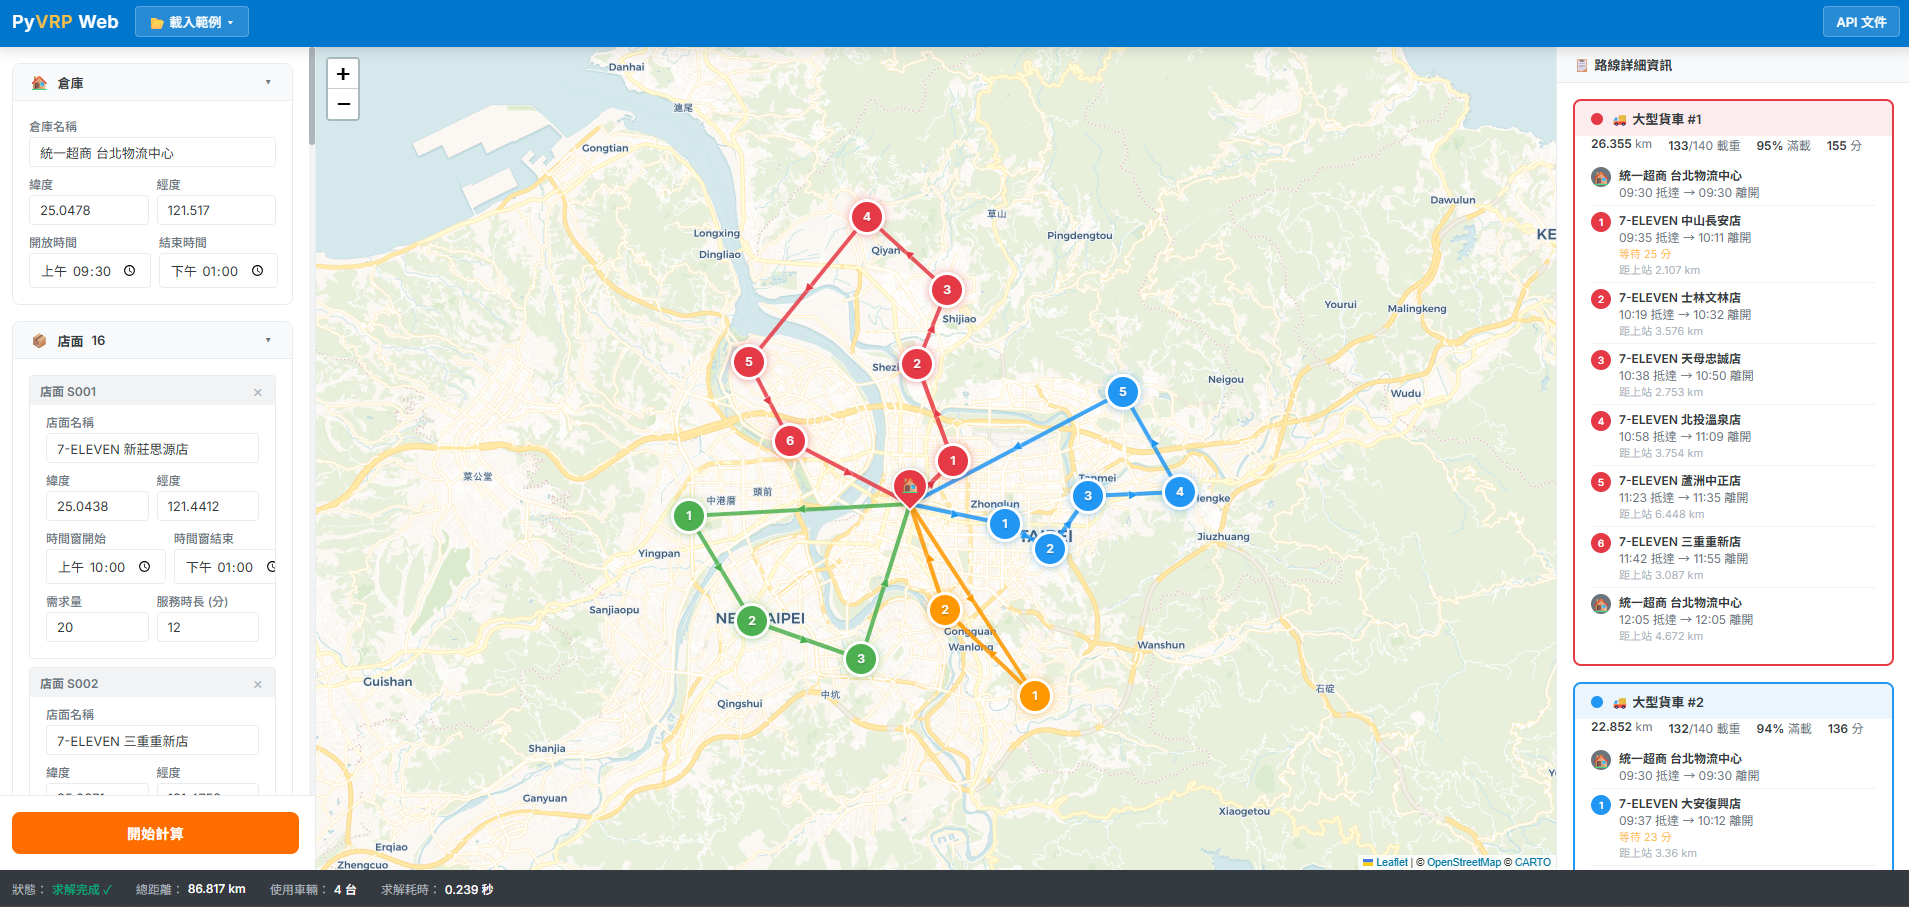
\includegraphics[width=\columnwidth]{figures/fig2_web_demo}
  \caption{PyVRP-Web interface showing optimized routes for the Taipei
           7-ELEVEN daytime distribution case study (16 stores, 3 routes,
           $\approx$92\,km). Color-coded routes with directional arrows and
           per-route timelines are shown.}
  \label{fig:webdemo}
\end{figure}

The web interface provides: real-time map visualization with directional
arrows, per-route timelines (arrival/departure/wait times), and
color-coded route highlighting with interactive selection.

% ── Section V: Conclusion ─────────────────────────────────
\section{Conclusion}

This paper presented a comprehensive study of \textbf{Hybrid Genetic
Search}---a state-of-the-art bio-inspired algorithm for the Vehicle Routing
Problem---and its implementation in PyVRP. We analyzed in depth the
biological analogy underlying HGS: SREX crossover mimics chromosomal
recombination, biased fitness implements natural selection with a diversity
premium to prevent premature convergence, and dynamic penalty management
acts as an environmental pressure steering the population toward feasibility.

Our implementation, \textbf{PyVRP-Web}, demonstrates that research-grade
bio-inspired optimization can be made accessible through modern web
technologies. Guided by a zero-intrusion encapsulation principle---leaving
PyVRP unmodified and wrapping all extensions in peripheral service
modules---the system resolves three practitioner barriers: coordinate system
incompatibility, neighbourhood size misconfiguration for small instances,
and the absence of per-stop timeline output. The system achieves near-optimal
routing solutions within seconds, validated by standard benchmarks (0.22\%
from BKS on CVRP) and a real-world Taipei distribution scenario.

Future directions include: (i) integrating real road network distances via
OSRM for travel time accuracy; (ii) supporting multi-depot VRP variants;
(iii) adding electric vehicle constraints (battery capacity, charging
stations); and (iv) visualizing the GA convergence trajectory in real time
to enhance educational value.

% ── References ────────────────────────────────────────────
\bibliographystyle{IEEEtran}
\bibliography{references}

\end{document}
